\begin{frame}[fragile]{Exemplos de funções unimodais}

    \begin{figure}
        \centering

        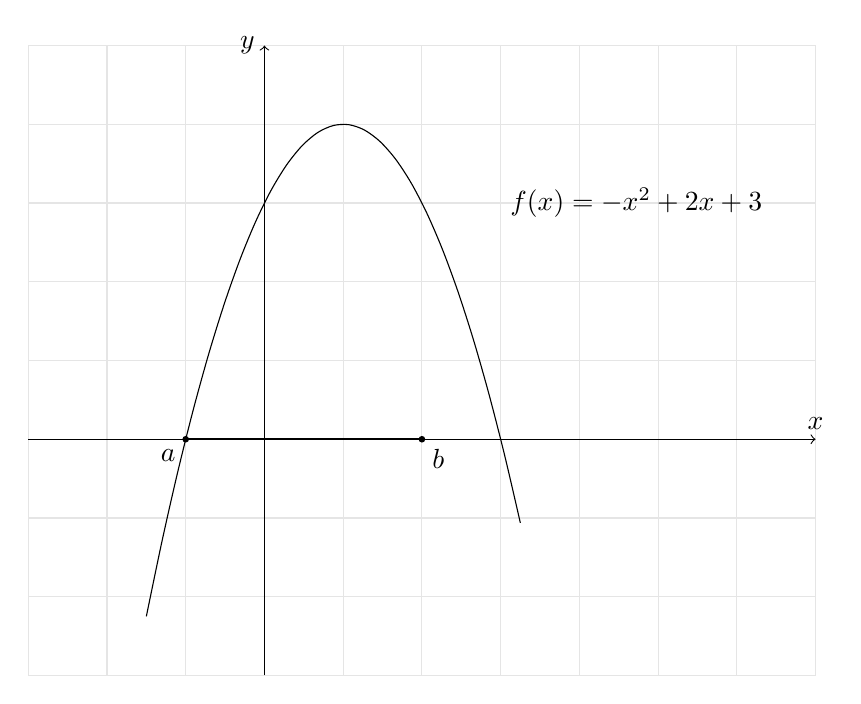
\begin{tikzpicture}
            \draw[gray!20] (-3, -3) grid (7, 5);

            \draw[smooth,domain=-1.5:3.25] plot (\x, {-\x*\x + 2*\x + 3});
            \node[anchor=west] at (3, 3) { $f(x) = -x^2 + 2x + 3$ };

            \draw[->] (0,-3) -- (0, 5) node[anchor=east] { $y$ };
            \draw[->] (-3,0) -- (7, 0) node[anchor=south] { $x$ };

            \draw[thick] (-1, 0) node[anchor=north east] { $a$ } -- (2, 0) node[anchor=north west] { $b$ };

            \fill (-1,0) circle [radius=1.2pt];
            \fill (2,0) circle [radius=1.2pt];
        \end{tikzpicture}
    \end{figure}

\end{frame}

\begin{frame}[fragile]{Exemplos de funções unimodais}

    \begin{figure}
        \centering

        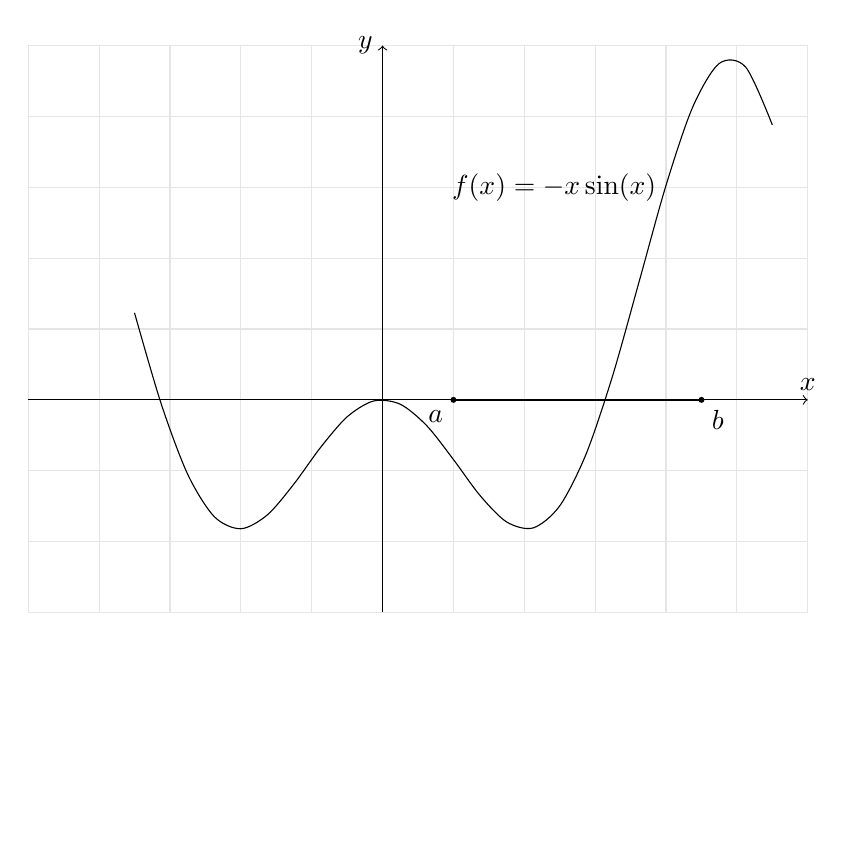
\begin{tikzpicture}
            \begin{scope}[scale=0.9]
                \draw[gray!20] (-5, -3) grid (6, 5);
                \draw[opacity=0] (0,-6);

                \draw[smooth,domain=-3.5:5.5] plot (\x, {-\x*sin(\x r)});
                \node[anchor=east] at (4, 3) { $f(x) = -x\sin(x)$ };

                \draw[->] (0,-3) -- (0, 5) node[anchor=east] { $y$ };
                \draw[->] (-5,0) -- (6, 0) node[anchor=south] { $x$ };

                \draw[thick] (1, 0) node[anchor=north east] { $a$ } -- (4.5, 0) node[anchor=north west] { $b$ };

                \fill (1,0) circle [radius=1.2pt];
                \fill (4.5,0) circle [radius=1.2pt];
            \end{scope}
        \end{tikzpicture}
    \end{figure}

\end{frame}
